
%%%%%%%%%%%%%%%%%%%%%%
%                                                                 %
% COMMERCIAL SOFTWARES REVIEW  %
%                                                                 %
%%%%%%%%%%%%%%%%%%%%%%

%COMMERCIAL SOFTWARES REVIEW
\chapter{Review of Available Geochemical Modelling Software}
\label{chapter:review}
The importance of geochemical models has increased lately due to the variety of applications, but the first models date back to the 70’s as can be observed \cite{Westall:76},~\cite{Wolery:79}. 
Since then, these models are used to solve problems as  speciation; determination of minerals' saturation indexes; adjustment of equilibrium for minerals; mixing of different waters; calculation of stoichiometric reactions; mixing of solids, fluids and gaseous phases; calculation of equilibrium/kinetic controlled reactions; reactive transport; and mass-law calculations.

The quality of the chemical analysis depend on the methods used, thermodynamic data and theoretical concepts applied. Therefore, it is crucial to verify the results and it is clear that there will be some differences in the results according to the software used. Among the enormous variety of software available, some of them are developed for batch-type simulations only, while others have transport capabilities. Several of them do not incorporate graphical interfaces and are written in FORTRAN, while newer distributions are mainly written in C/C++ and, due to proprietary reasons, code is not distributed with the software. Ii ts important to mention that, even in those who provide an integrated graphical user interface (GUI), it is often very tedious and time-consuming to generate input files for groundwater simulation.

The goal of this chapter is to review other programs that perform modelling of aqueous geochemical systems. It is not possible nor the purpose of this work to present all the existing software but to critically review and compare some aspects of them. These systems are being widely used by the community and have enough documentation published as open literature that makes a comparison doable without much effort. 

In this work, only programs that provide speciation modelling are reviewed. They are the following: \emph{EQ3/6}; \emph{PHREEQC}; \emph{MINTEQ}; and \emph{SOLMINEQ};

We will present relevant detail about the geochemical point of view and then, we will critically analyze and discuss each software from the computer science point of view. It's worth mentioning that sometimes is not possible to analyse the same aspects of different softwares due to lack of information.


%GEOCHEMICAL SPECIATION MODELLING CODES
%\section{Geochemical Speciation Modelling Software}

%EQ3/6
\section{\emph{EQ3/6}}
EQ3/6 consists of two programs: EQ3 is a pure speciation code whose results EQ6 subsequentially process. It is a software package for geochemical modeling of aqueous systems written in FORTRAN77. EQ3/6 includes a speciation-solubility solver, which is useful for analyzing groundwater chemistry data, calculating solubility limits and determining whether certain reactions are in states of partial equilibrium or disequilibrium. It also offers a reaction path calculation that models water/rock interaction or fluid mixture. EQ3/6 supports several thermodynamic data files (these data files contain support for Davies, B-dot, Debye-Hueckel equations, as well as support data for standard state and activity coefficient-related). It is developed to run under UNIX, and the full package distribution is not free (it requires a license) \cite{Wolery:79} \cite{Wolery:90} \cite{Wolery:92}.

\subsection{Input/Output Options}
The \emph{datafilekey} and \emph{inputfile} given to the program as arguments must be consistent with the options and methods. For example, if they have different methods for calculating the activity coefficient there will be problems, and the results will be meaningless. Another point to be taken into consideration and that follows the same idea, the \emph{inputfile} must be using chemical data (for example, elements, species and compounds) that is known by the \emph{datafilekey}.

Inside each file, there are a series of \emph{blocks} that are combined to support the geochemical speciation. They are presented bellow:
\begin{itemize}
\item \emph{Datafilekey}: Title; Miscellaneous parameters (temperature limit, activity coefficient parameters, pressure); chemical elements block; qqueous species block; pure minerals block; pure non-aqueous liquids block; gas species blocks; solid solutions blocks; references blocks
\item \emph{Inputfile}: Title; Special basis switches; temperature; pressure option; density; total dissolved salts (TDS) option; electrical balancing option; redox option; basis species constraints; ion exchanger creation flag; ion exchanger compositions; solid solutions compositions; alter/suppression options; iopt options; iopg options; iopr options; iodb options; numerical parameters; ordinary basis switches; saturation flag tolerance; aqueous phase scale factor.
\end{itemize}

EQ3/6 package produces different outputs depending on the software that is used. We will exemplify the output files in general by using the \emph{EQ3NR} and \emph{EQ6} output formats. 
\begin{itemize}
\item \emph{EQ3NR}: Two output files are generated: a \emph{pickup} file and the normal output file. The \emph{pickup} file can be used as input to \emph{EQ6} software. The normal output file consists of six blocks: header section; input file echo; recap of input data; iterative calculations; principal results; and finally the end of EQ3NR run
\item \emph{EQ6}: This program generates three output files: a \emph{tab} output file, a \emph{pickup} output file and the normal output file. The \emph{tab} file contains information that can be used to plot output results. The \emph{pickup} file is the input to \emph{EQ6}. The normal output file consists of six \emph{blocks}: header; input echo; input recap; iterative calculations; principal results; and the end of \emph{EQ6} run.
\end{itemize}

A small excerpt of an \emph{EQ6} outpuf file is shown in code ~\ref{eq3:output}.

\begin{minipage}[c]{0.92\textwidth}
\begin{lstlisting}[frame=single, caption=Excerpt of \emph{EQ6} output file, label=eq3:output]
...
 Entity Date Base Dimension Current Problem
 Chemical Elements 81 81 6
 Basis Species 201 259 7
 Phases 1135 1159 29
 Species 3031 3523 0
 Aqueous Species 1769 1769 22
 Pure Minerals 1120 1120 26
 Pure Liquids 1 3 1
 Gas Species 93 93 2
 Solid Soutions 12 12 0
...
\end{lstlisting}
\end{minipage}

\subsection{User Interaction}
In \emph{EQ3/6} the command prompt is used for all the user interaction. There are several functions inside \emph{EQ3/6}; the appropriate command will trigger each one of them. From the existing software, there are \emph{EQ3NR}, \emph{EQ6} and \emph{EQPT} just to name a few. The user must enter the command from the keyboard and must use this "command prompt". By pressing "CTRL+C" at any time the execution stops, literally "breaking" the process. For example, EQ3 is run by commands of the form shown in code ~\ref{eq3:run}.

\begin{lstlisting}[frame=single, caption=Running EQ3 in \emph{EQ3/6} package, label=eq3:run]
>runeq3 datafilekey inputfile(s)
\end{lstlisting}

In this command, \emph{datafilekey} and \emph{inputfile} are arguments, being the former a three-character identification associated to which database should be used, while the latter is specifically the name of the input file, which can be more than one. Depending on which program from the package the user is using, it generates from two to several output files (always in the \emph{ASCII} format).
As mentioned, the input file will be entered in the program as an argument. Any regular text editor is sufficient to create or modify an input file (although it is not recommended that the user create an input file from scratch). There are several pre-existing input templates available and, if none of them matches the need of the user, \emph{EQ3/6} recommends that the user generate a new one by copying existing blocks from any provided template.

The input files can contain instructions/parameters that try to recreate known user interactions method as shown in code ~\ref{eq3:menu}.

\begin{minipage}[c]{0.92\textwidth}
\begin{lstlisting}[frame=single, caption=Menu Option inside \emph{EQ3/6} input files that mimics a "radio button", label=eq3:menu]
iopr(4) - Print a Table of Aqueous Species Concentrations, Activities, etc.: 
 [ ] (-3) Omit species with molalities < 1.e-8 
 [ ] (-2) Omit species with molalities < 1.e-12 
 [ ] (-1) Omit species with molalities < 1.e-20 
 [x] ( 0) Omit species with molalities < 1.e-100 
 [ ] ( 1) Include all species 
\end{lstlisting}
\end{minipage}

% VEJA E-MAIL SOBRE ESSE TEXT FILE QUE É DATABASE ABAIXO 
% Reformatei todo o paragrafo, tirando o foco do especifico problema de text/binary, mas salientando que o uso desse tipo de arquivo acaba gerando desperdicio de memoria que é importante... a ideia permanece a mesma, mas com outro appraoch..deixando bem claro em qualquer linguagem, eu imagino..
\subsection{File Formats}
All the files discussed above are \emph{ASCII} text files and, therefore, any regular text editor can be used to edit or build them. When the text file contains thermodynamic informations needed by the program, the whole group of information is copied to the memory and, only after that, the software will be able to fetch information and continue the simulation's processing and natural flow. In memory, the storage of this information is not always optimized, specially because \emph{ASCII} files are, in general, also not very well organized. Waste of memory here and there are expected and usual in this kind of text and memory management - scale this to a large amount of \emph{ASCII} information - like in geochemical modelling systems - and it is easy to understand the risk that comes together with \emph{ASCII} text files. 

% TENHO DUVIDA - ACHO QUE NÃO PRECISA ESSA SEÇÃO DE INSTALAÇÃO
\subsection{Software Environment and Installation Procedures}
The \emph{EQ3/6} package runs on Windows (95 and upper versions) and was developed in FORTRAN77. The support for UNIX computers has been discontinued.  It has been developed and run at Lawrence Livermore National Laboratory on an Alliant FX/80 and Sun SPARCstations.

The installation of \emph{EQ3/6} is explained in details in \cite{Wolery:92}. Due to the purpose of this work, details of the installation will be suppressed here. At the same time, it is interesting to mention that the whole installation process requires some level of experience with command prompt and \emph{DOS}.



%PHREEQC
\section{\emph{PHREEQC}}
\emph{PHREEQC} stands for \emph{PH} \emph{RE}dox \emph{EQ}uilibrium in \emph{C} language, and is a widely used public-domain geochemical modelling software available from the USGS  \cite{Parkhurst:80}, available for download in versions for PC and Mac. It was designed to perform a wide variety of low-temperature aqueous geochemical calculations based on an ion-association aqueous model and has capabilities to:
\begin{itemize}
\item Speciation and Saturation Index calculations;
\item Batch reaction and one-dimensional (1D) transport calculations involving reversible reactions (including aqueous, minerals, gas, solid-solution, surface-complexation, and ion-exchange equilibrium) and irreversible reactions (including specified mole transfer of reactants, kinetically controlled reactions, mixing of solutions and temperature changes);
\item Inverse modelling, which finds sets of mineral and gas mole transfers that takes into account differences in composition between waters.
\end{itemize}

\subsection{Input/Output Options}
The input data for \emph{PHREEQC} is arranged by \emph{keyword data blocks}. Each block is organized with a keyword in the first line, followed by lines containing data related to the keyword. Keywords and their respective contexts are read from the database at the beginning of the run to define all the necessary parameters. After this database reading procedure, it will continue reading the input file until the it reaches the \emph{END} keyword. As the input file is being read, the program will start putting the pieces together to perform the necessary calculations. An example of a \emph{keyword data block} is shown in code ~\ref{phreeqc:keyword}. Among the possible keywords available in \emph{PHREEQC} are EQUILIBRIUM PHASES, EXCHANGE, GAS PHASE, INVERSE MODELING, PHASES, REACTION, PRINT, SAVE, SOLUTION SPECIES, etc. Each one of these keywords contains specific arguments and parameters to be used. Certain keywords require some other specific keywords, and if something is missing from the input file, the results will be inconclusive and wrong. So building an input file is usually quite difficult. 

\begin{minipage}[c]{0.92\textwidth}
\begin{lstlisting}[frame=single, caption=\emph{PHREEQC} keyword data block example, label=phreeqc:keyword]
EQUILIBRIUM_PHASES
Chalcedony  0.0     0.0
CO2(g)      -3.5    1.0
Gibbsite(c) 0.0     KAlSiO8  1.0
Calcite     1.0     Gypsum   1.0
pH_Fix      -5.0    HCl      10.0
\end{lstlisting}
\end{minipage}

The output file will contain the results of the simulation defined in the input file also divided into \emph{keyword blocks}. Among those, we can mention solution composition, description of the solution, redox couples, distribution of species (as can be seen in code ~\ref{phreeqc:output}), and saturation indices.

\begin{minipage}[c]{0.92\textwidth}
\begin{lstlisting}[frame=single, caption=\emph{PHREEQC}'s excerpt from the output file, label=phreeqc:output]
...
----------------------------Distribution of species----------------------------
 
                                               Log       Log       Log    mole V
   Species          Molality    Activity  Molality  Activity     Gamma   cm3/mol
 
   OH-            2.705e-006  1.647e-006    -5.568    -5.783    -0.215     -2.63
   H+             7.983e-009  6.026e-009    -8.098    -8.220    -0.122      0.00
   H2O            5.551e+001  9.806e-001     1.744    -0.009     0.000     18.07
C(4)         2.257e-003
   HCO3-          1.238e-003  8.359e-004    -2.907    -3.078    -0.170     27.87
   NaHCO3         6.168e-004  7.205e-004    -3.210    -3.142     0.067     19.41
   MgHCO3+        2.136e-004  1.343e-004    -3.670    -3.872    -0.201      5.82
   MgCO3          7.301e-005  8.527e-005    -4.137    -4.069     0.067    -17.09
   CaHCO3+        3.717e-005  2.572e-005    -4.430    -4.590    -0.160      9.96
   CO3-2          3.128e-005  6.506e-006    -4.505    -5.187    -0.682     -0.34
   CaCO3          2.256e-005  2.636e-005    -4.647    -4.579     0.067    -14.60
   NaCO3-         1.477e-005  9.972e-006    -4.831    -5.001    -0.170      1.77
...
\end{lstlisting}
\end{minipage}

\subsection{User Interaction}
\emph{PHREEQC}'s distribution differs drastically according to the environment (\emph{Windows} or \emph{UNIX}). By this reason, the analysis of user interaction features will be done separately.

\begin{itemize}
\item \emph{PHREEQC} for Windows: Due to the need of a geochemical modelling software and the lack of interface for \emph{PHREEQC} in the first versions of the software, many efforts were done to create an interface to \emph{PHREEQC}. The program \emph{PhreeqcI} is a graphical user interface to \emph{PHREEQC} that provides data entry screens for the keyword data blocks with a description of each input data item. It organizes the input file by using some \emph{project tree} which facilitates viewing, selecting, editing and running the \emph{PHREEQC} simulations. It is critical to mention that \emph{PhreeqcI} does not implement all the keyword blocks. After this, another effort was done and \emph{PHREEQC} version 2 with a graphical interface was launched, the interface being kept later in version 3. This graphical interface was baptized \emph{PfW} (Phreeqc for Windows) but it has no updates since 2011. It can be seen in Figure ~\ref{fig:phreeqc-pfw}. The last effort in this sense was the development of an adaptation of the popular general-purpose text editor \emph{Notepad++}. This modification comes with the following capabilities: syntax highlighting; autocompletion of keywords and identifiers; tips; colored numbers; parenthesis matching; commenting and uncommenting multiple lines at once; column editor; few shortcuts; and file recognition; This can be seen in Figure ~\ref{fig:phreeqc-notepad++}. When running PHREEQC from the \emph{Notepad++} adaptation, the command prompt is called and the simulation is executed, as in Figure ~\ref{fig:phreeqc-notepad++2}. There are some options and shortcuts available from the \emph{Notepad++}'s interface, which is shown in detail in Figure ~\ref{fig:phreeqc-notepad++3}.
\item \emph{PHREEQC} for UNIX: Under UNIX's distribution, \emph{PHREEQC} runs from the command prompt. It can be launched by using the command shown in code ~\ref{phreeqc:run}
\begin{lstlisting}[frame=single, caption=Command to run UNIX's \emph{PHREEQC}, label=phreeqc:run]
phreeqc input output database screen_output
\end{lstlisting}
The \emph{"input"} file contains the description of the simulation, the \emph{"output"} file will store the results of the simulation, \emph{"database"} specifies which database should be used, and \emph{"screen\_output"} stores the information that will be shown on screen. If the user does not specify the names of \emph{"output"}, \emph{"database"} or \emph{"screen\_output"} the geochemical modelling software will choose default values.
\end{itemize}

\begin{figure}[ht!]
\centering
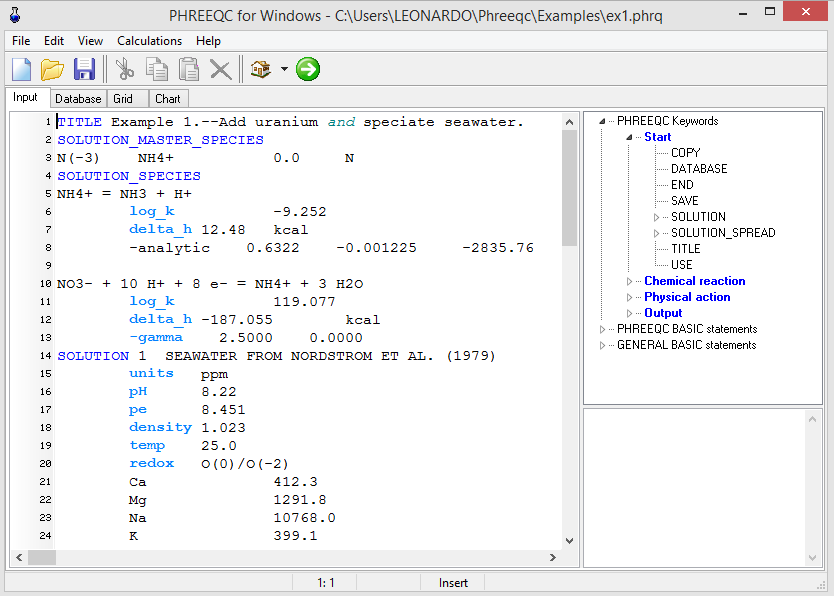
\includegraphics[width=100mm]{figures/pfw.png}
\caption{User interface of the PHREEQC for Windows (\emph{PfW})}
\label{fig:phreeqc-pfw}
\end{figure}

\begin{figure}[ht!]
\centering
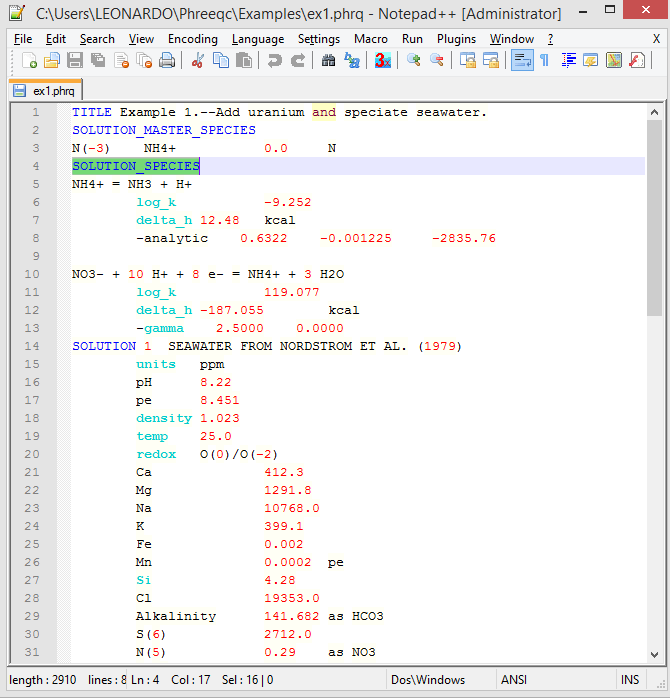
\includegraphics[width=100mm]{figures/notepad++Phreeqc.png}
\caption{Example of the PHREEQC Notepad++ plugin}
\label{fig:phreeqc-notepad++}
\end{figure}

\begin{figure}[ht!]
\centering
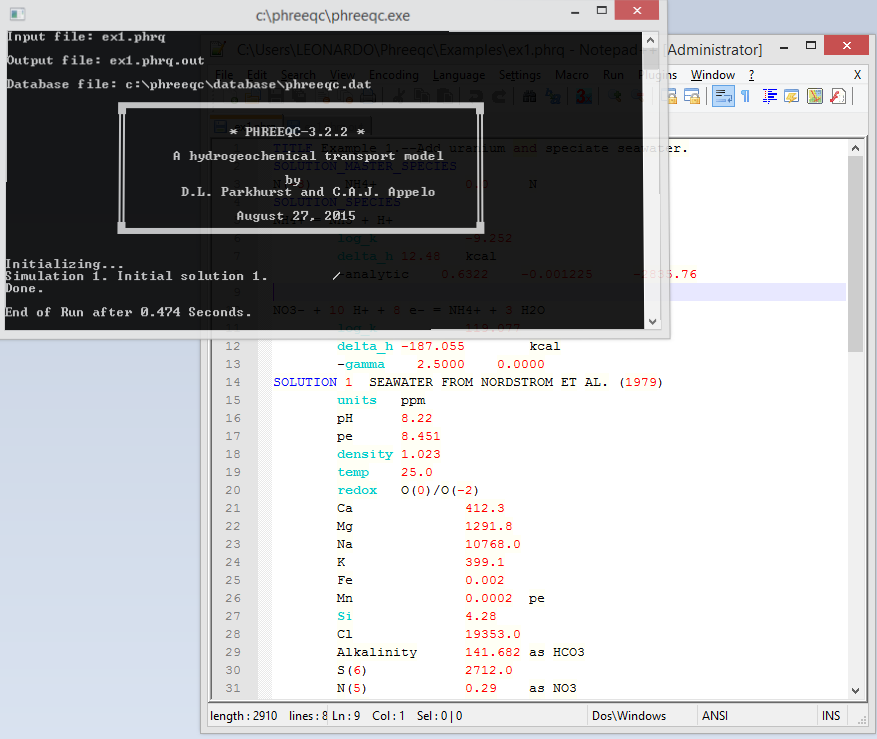
\includegraphics[width=100mm]{figures/notepad++PhreeqcProcess.png}
\caption{PHREEQC software called from the Notepad++ Plugin}
\label{fig:phreeqc-notepad++2}
\end{figure}

\begin{figure}[ht!]
\centering
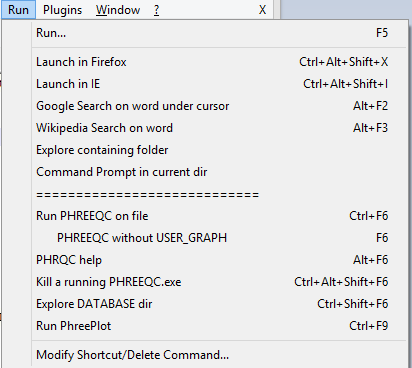
\includegraphics[width=100mm]{figures/notepad++run_menu.png}
\caption{PHREEQC software called from the Notepad++ Plugin}
\label{fig:phreeqc-notepad++3}
\end{figure}

\subsection{File formats}
All the files discussed above are in the \emph{ASCII} text files format and, therefore, any regular text editor can be used. 
It is recommended that the editing of \emph{PHREEQC} files be done by using the NotPhreeqcce or notepad++ adapted version \cite{NotPhree:11}.

% IDEM - ACHO DESNECESSÁRIO
\subsection{Software Environment and Installation Procedures}
\emph{PHREEQC} has support for Windows (32 and 64-bit), MacOS (OS 10.6+) and Linux. \emph{PHREEQC} is currently on version 3 and with frequent updates, bug fixes and maintenance.

The \emph{PHREEQC} version for Windows has a self-extracting file that can is available for download from the USGS website and easily installed. The \emph{UNIX} distribution comes with additional scripts and a makefile and the user should follow some steps to compile and install the program.

%MINTEQ
\section{\emph{MINTEQ}}
\emph{MINTEQ} is a geochemical program to model aqueous solutions and the interactions of aqueous solutions with hypothesized assemblages of solid phases. It has a particular inclination to calculate equilibrium composition of dilute aqueous solutions. The model is useful for calculating the equilibrium mass distribution among dissolved species, adsorbed species and multiple solid phases although it has a much simpler treatment of the reactions. 

It was originally developed in FORTRAN77 by Battelle Pacific Northwest Laboratory (\emph{PNL}) and continued by the Environmental Protection Agency (\emph{EPA}) to perform the  necessary calculations regarding waste, sediments and ground water. \emph{MINTEQ} does not consider the kinetic reactions and works at fixed temperature ($25$ degrees Celcius). 
An extensive database adequate to a broad range of problems is part of the software, and there is no need for the user to change nor add anything \cite{Brown:87} \cite{Allison:91}. The latest update on \emph{MINTEQ} dates from 1990, and since then, there has been only some improvements especially on the usability and calculations. This version was named \emph{MINTEQA2} and uses a well-developed thermodynamic database from the \emph{USGS}.

\subsection{Input/Output Options}
The input files for \emph{MINTEQA2} can be generated manually, but there is another software called \emph{PRODEFA2} that guides the user to accomplish this task. \emph{PRODEFA2} is an interactive program used to create input files that will be addressed in details in section ~\ref{minteq:interactions}. Four parts compose the input file:
\begin{itemize}
\item Input file: The input file that contains the data input by the user. Typically, this file contains dissolved (i.e. Ca concentrations, pH, temperature) and solid phase (i.e. minerals, sorption sites) information for a water sample;
\item Database file: This file contains the thermodynamic constants that govern the processes of interest (i.e. complexation constants, mineral solubilities, activity constants) which will be used to conduct calculations;
\item Algorithm or executable file:  These files contain the algorithms of the code, which solve the specified problem (usually using an iterative numerical approach) within the constraints imposed by the Database files and the information in the Input file.
\item Output file: This file contains the results of the calculations performed by the Algorithm Files.
\end{itemize}

Among the input file's options, there are four levels of configuration. Each level controls some details of the simulation, and when these four levels are together, they compose a complete input file for \emph{MINTEQA2}. Important to mention that if the user does not want to specify all the details for every level, there are default options that enable any non-experienced user to execute simple simulations.
\begin{enumerate}
\item Displays the current settings of system parameters such as temperature as well as program flag settings such as the number of iterations allowed;
\item Specify the chemistry of the system;
\item This level works as a "line editor" in displaying by category or TYPE those species that have been explicitly entered through level 2;
\item Deals with utility functions (output file details, for example);
\end{enumerate}

If database, algorithm and output files are not specified, default options are used. Code ~\ref{minteqa2:input}  brings the \emph{MINTEQA2}'s input file used in the study case discussed in chapter~\ref{chapter:validation} and presented here as example. The beginning of the file (first and second lines) contains  a description of the simulation or input file; the third, fourth and fifth line brings settings configuration: details as temperature, unit chosen, eH, ionic strength, number of iterations, precipitation options. After that, comes the components that take part in the simulation, organized by internal id, concentration details and log of concentration;

\begin{minipage}[c]{0.92\textwidth}
\begin{lstlisting}[frame=single, caption=\emph{MINTEQA2}'s input file, label=minteqa2:input]
LHDAMIANI - STUDY CASE
Comparative study           
25.00 MOLAL  0.000  0.00000E+00
0 0 1 0 1 0 0 0 1 1 0 0 0
0   0   0
    330  6.026E-09   -8.22 y                    /H+1               
    410  1.045E-02   -1.98 y                    /K+1               
    500  4.793E-01   -0.32 y                    /Na+1              
    150  1.053E-02   -1.98 y                    /Ca+2              
    460  5.439E-02   -1.26 y                    /Mg+2              
    732  2.889E-02   -1.54 y                    /SO4-2             
    180  5.595E-01   -0.25 y                    /Cl-1              

\end{lstlisting}
\end{minipage}



An excerpt of \emph{MINTEQA2}'s output is presented in Code ~\ref{minteqa2:output}. The whole output file is divided into six parts:
\begin{enumerate}
\item Reproduction and interpretation of the input file;
\item Detailed listing of species read from the database files;
\item Iteration information and detailed information for each specie;
\item Percentage distribution of components among dissolved and adsorbed species;
\item Provisional or equilibrated mass distribution, provisional or equilibrium ionic strength, equilibrium pH and pE, electrostatic surface potencial and charge for electrostatic adsorption models;
\item Saturation indices for all database solids with respect to the solution;
\end{enumerate}


\begin{minipage}[c]{0.92\textwidth}
\begin{lstlisting}[frame=single, caption=\emph{MINTEQA2}'s excerpt from the output file, label=minteqa2:output]
...
_______________________________________________________________________
______________________________ PART 3 of OUTPUT FILE __________________
  MINTEQA2  v4.02   DATE OF CALCULATIONS:  5-JUN-2000  TIME: 14: 6:27



PARAMETERS OF THE COMPONENT MOST OUT OF BALANCE:

ITER      NAME       TOTAL mol/L   DIFF FXN   LOG ACTVTY    RESIDUAL
0   SO4-2           1.580E-03   6.594E-07    -2.91757    5.014E-07
1   SO4-2           1.580E-03   4.193E-04    -2.91775    4.192E-04
2   SO4-2           1.580E-03   8.125E-06    -3.01997    7.967E-06
3   SO4-2           1.580E-03   1.693E-07    -3.02220    1.135E-08

 ID No  Name        Total Conc(M)    Conc (M)  log Activity   Diff fxn
  410   K+1            7.700E-05     7.649E-05    -4.14759    5.093E-11
  732   SO4-2          1.580E-03     1.266E-03    -3.02224    3.557E-09
    2   H2O            0.000E+00    -1.049E-05    -0.00004    0.000E+00
  330   H+1            0.000E+00     3.398E-03    -2.50000    0.000E+00
  140   CO3-2          0.000E+00     2.916E-17   -16.66004    0.000E+00

-----------------------------------------------------------------------
...
\end{lstlisting}
\end{minipage}

\subsection{User Interaction}\label{minteq:interactions}
\emph{MINTEQA2} and \emph{PRODEFA2} interactions are completely independent programs and \emph{PRODEFA2} is used before \emph{MINTEQA2} in order to generate the input file that will be consumed by the latter. Everything is done through the command prompt and on this work will detail \emph{PRODEFA2}'s interaction. It provides a "walk-through" to generate an input file for \emph{MINTEQA2}.

After opening the software and providing a valid name, it will ask which part of the input file the user wants to create or edit as shown in figure ~\ref{minteq:init}. We will follow the suggested order and go through 4 levels, as previously discussed in this section. Figure ~\ref{minteq:level0} shows the main menu, it is the organization of all the levels and works as a central hub of information. Figure ~\ref{minteq:level1} displays the necessary information about level 1,     in order to change any of the entries on this screen, the user must enter the number to the left of the entry and respond to the questions presented. All the four levels do this kind of interactions. Through these interactions, the user has access to all the information in the database and can choose specifically about what is the model.

\begin{figure}[ht!]
\centering
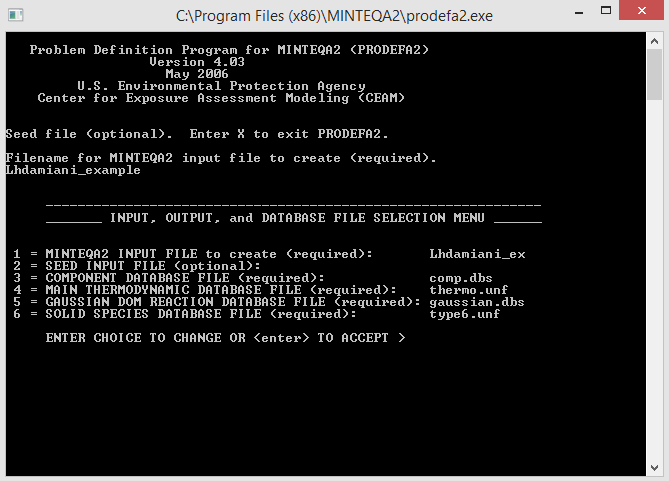
\includegraphics[width=100mm]{figures/minteq-init.png}
\caption{\emph{MINTEQA2} initial menu options}
\label{minteq:init}
\end{figure}

\begin{figure}[ht!]
\centering
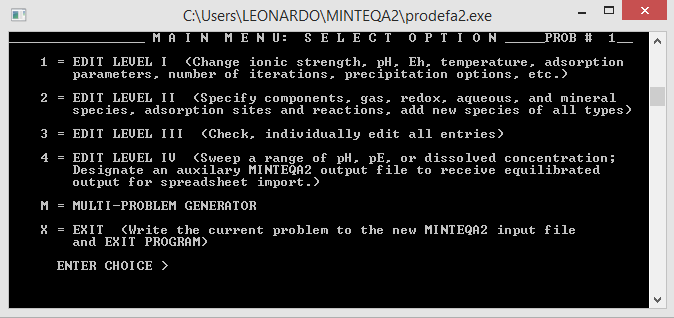
\includegraphics[width=100mm]{figures/minteq-level0.png}
\caption{\emph{MINTEQA2} main menu}
\label{minteq:level0}
\end{figure}

\begin{figure}[ht!]
\centering
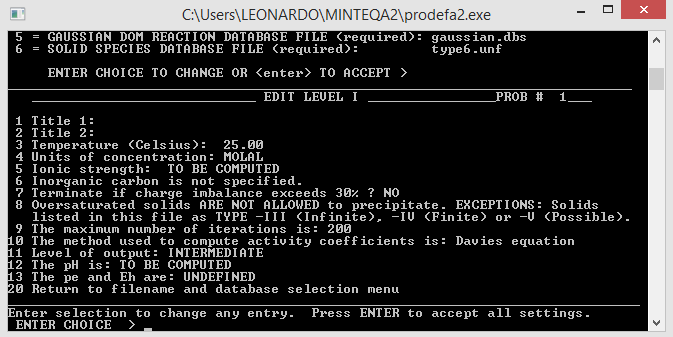
\includegraphics[width=100mm]{figures/minteq-level1.png}
\caption{\emph{MINTEQA2} Level 1 informations}
\label{minteq:level1}
\end{figure}


During this work, we chose to add a specific aqueous specie to show the \emph{PRODEFA2} interactions and present it step-by-step bellow:

\begin{enumerate}
\item Choose level 2 on main menu;
\item Choose option 1 (Specify AQUEOUS COMPONENTS: TOTAL CONCENTRATIONS or FIXED ACTIVITIES) inside the menu from level 2;
\item Choose option 1 (TOTAL DISSOLVED CONCENTRATION), it identifies how we want to entre this new component.
\item At this step, we are requested to enter the first letter for the component. Alternatives to this approach is to enter "-1" if you know the components id number or quit. We will add \ce{Na^+} to the system. So, we type the letter "N" and hit enter button.
\item At this step, all the existing options available are shown listed with an identifier and we are requested to identify which one of these we want to add. This can be seen in ~\ref{minteq:Na+}.
\item After pressing \ce{Na^+}'s id (at this case was the number 4). We can finally enter the TOTAL DISSOLVED CONCENTRATION (MOLAL) of COMPONENT. Defined earlier on step 3 After adding the molal concentration for this specie the system goes back to step 4 in case we want to continue adding other components.
\end{enumerate}

\begin{figure}[ht!]
\centering
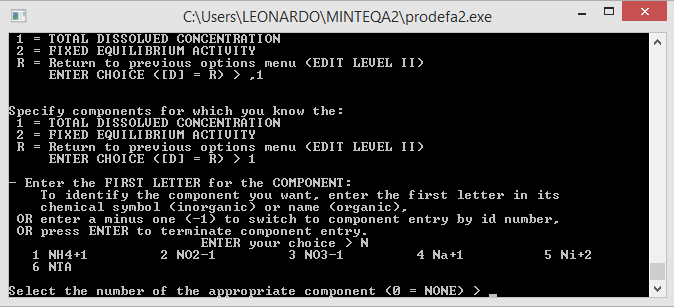
\includegraphics[width=100mm]{figures/minteq-Na+.png}
\caption{\emph{PRODEFA2}'s example of adding a specific aquoues specie (\ce{Na+}) }
\label{minteq:Na+}
\end{figure}

There is also a software called \emph{Visual Minteq} that tries to "humanize" \emph{MINTEQ} and was maintained by the KTH Royal Institute of Technology, located in Stockholm, Sweden. \emph{Visual Minteq} latest release date is December 2013 at the version 3.0 and is available only for \emph{Windows} operating systems since it was developed in Visual Basic. 

\subsection{File formats}
All the files follow a regular text format (\emph{ASCII}) and their purpose is defined on the extension of the file. 
\begin{itemize}
\item Input files have the extension \emph{"INP"};
\item Test and help files have the extension \emph{"HLP"};
\item Output files have the extension \emph{"LST"};
\item Database files have the extension \emph{"DBS"} or \emph{"UNF"};
\item Input file have the extension \emph{"INP"};
\end{itemize}


% Juntei as duas partes como tu sugeriu.. deixei a parte de installation procedures .. qualquer coisa posso tirar depois se decidirmos nao utilizar.
\subsubsection{Software Environment and Installation Procedures}
It is currently at the version 4.03 (Windows only), interesting to mention that this release date back to May 2006. The latest \emph{UNIX} distribution is version 3.12 (which was also called BETA for UNIX) and date back to August 1996.
\emph{MINTEQA2} is easily installed by a self-extractor installer that can be downloaded from \emph{EPA}'s website \cite{minteq:website} and \cite{minteq:unix}. Included in the distribution package are also some important documentation, \emph{PRODEFA2} software and several input/output template files.
The UNIX version distribution comes with the source files and must be compiled to run.



\section{\emph{SOLMINEQ.88}}
\emph{SOLMINEQ.88} is an FORTRAN 77 written geochemical modeling program based on SOLMNEQ \cite{Kharaka:73} with improved algorithms that result in a faster program execution and tighter convergence. The software has a database with the focus on organics aqueous species. It calculates the distribution of mass among aqueous species and complexes and calculates saturation indexes of minerals at different temperatures and pressures. It includes options as boiling, mixing of solutions and partitioning of gases between water, oil and a vapour phase. \emph{SOLMINEQ.88} also contemplates mass transfer with the effects of dissolution and precipitation of minerals and options to calculate activity coefficient model \cite{Kharaka:88}. The original version has no UI, but there were further studies with the intention of creating a user-friendly program that can be used to generate, edit and analyze input and output files - \emph{SOLINPUT}.
\emph{SOLMINEQ.88} model has not been developed any further nor improved since its first release.

\subsection{Input/Output Options}
The input of \emph{SOLMINEQ.88} consists of two sets of data: fixed and variable. The first contains the chemical composition of an aqueous fluid and options for processing these data; and the last Consists of input data required for using them.

The input file is composed by six parts, \emph{SOLINPUT} guides the user throught all of them:
\begin{enumerate}
\item Basic Parameters: enter the chemical and physical data for that sample;
\item Flags: controls how the software interprets, process and display the data;
\item pH: controls the details of how the pH calculation is done;
\item Mass transfer: defines which mass transfer capabilities are used;
\item User Log K: make temporary changes and extensions to the database;
\item Additional ions and minerals: temporarily adds user defined ions and minerals to a particular simulation;
\end{enumerate}

The output file contains the results of the computations by \emph{SOLMINEQ.88} and it consists of six parts: An input data echo that shows the values and options selected for each sample; A table listing the calculated tolerance factor for successive iterations on the anions; A list of input to \emph{SOLMINEQ.88} including sample description, pH, Eh, temperature and os on; A table showing the distribution of species in solution; Ratios of a number of cations and anions of importance in geochemical processes; and th
e last one contains a table indicating the states of reactions for minerals considered;

\begin{minipage}[c]{0.92\textwidth}
\begin{lstlisting}[frame=single, caption=\emph{SOLMINEQ.88}'s excerpt from the output file, label=solmineq:output]
 : Test Sample #1 for SOLMINEQ.88 - Modified Seawater at 25 C
TEMP HI TEMP DENS PRESS
0.2500E+02 O.OOOOE+00 0.1023E+01 O.OOOOE+00
PH EHM EHMC EMFZSC
0.8200E+01 0.5000E+00 0.9000E+01 0.9000E+01
CONCENTRATION UNITS : PPM
Na K Li Ca
0.1077E+05 0.3991E+03 0.1810E+00 0.4123E+03
Si02 Cl S04 H2S
0.4280E+01 0.1935E+05 0.2712E+04 O.OOOOE+00
F P04 N03 NH3
0.1390E+01 0.6000E-01 0.2900E+00 0.3000E-01
Pb Zn Cu Mn
0.5000E-04 0.4900E-02 0.7000E-03 0.2000E-03
As U V
0.4000E-02 O.OOOOE+00 O.OOOOE+00
Acetate Oxalate Succinate CH4
0.1000E+00 0.1000E+00 0.1000E+00 0.1000E+00
\end{lstlisting}
\end{minipage}

\subsection{User Interaction}
The software that accompany \emph{SOLMINEQ.88} and handles the generation of input files and all the interactions is named \emph{SOLINPU} and described in \cite{Debraal:89}. All the interactions use the command prompt - the menus with several options are generated and displayed. The user selects the option by entering the indication number and pressing enter (the indication number stays on the left of the option). Figure ~\ref{solmineq:interaction} shows this example of interaction.

\begin{minipage}[c]{0.92\textwidth}
\begin{lstlisting}[frame=single, caption=\emph{SOLMINEQ.88}'s example of user interaction, label=solmineq:interaction]
	pH OPTIONS
1) Gas Addition Option
2) Gas-Water-Oil Distribution Option
3) Carbonate Mineral Saturation Option
4) C02 Option
5) Tolerance factor for Mineral and C02 Options
6) Return to Options Menu
Enter Choice (1-6)   __
\end{lstlisting}
\end{minipage}

\subsection{File formats}
The input files are regular \emph{ASCII} text files and any regular text editor is good for creating or editing.The database files from \emph{SOLMINEQ.88} have the extension "TBL" and the output files 


%Mesma coisa, juntei as duas partes e qualquer coisa tiro depois se decidirmos cortar fora mesmo..
\subsection{Software Environment and Installation Procedures}
As mentioned, \emph{SOLMINEQ.88} had only one release and has been discontinued since then. It is available only for the \emph{Windows} operating system.

SOLMINEQ.88 distribution requires knowledge in compiling and linking FORTRAN77 programs. It also comes with the software \emph{SOLINPUT} that makes the user interactions, as explained before, easier.

Interesting to point that along the installation manual, they recommend  that curious compiling options are activated, for example \emph{"do not check for array bounds"}, and \emph{"do not check subprogram interfaces"}.

%GEOCHEMICAL SPECIATION ANALYSIS
\section{Discussion}
On this section we compare, analyze and discuss some important aspects and issues of each one of the software presented earlier in this work. Regarding geochemical features, table ~\ref{tab:comparativeTable} brings certain aspects and features of the software.

\begin{table}
\caption{Geochemical comparison between speciation softwares}
\label{tab:comparativeTable}
\centering
\begin{tabular}{r|cccccccc}
SOFTWARE &
\rot{Aqueous Complexation} &
\rot{Precipitation and Dissolution Mass Balancing} & 
\rot{Reaction path} &
\rot{Kinetics} &
\rot{Multi-Activity Coefficient methods} 
    \\ \hline
EQ3/6        	&  \OK &  \OK & \OK & \OK & \OK    \\ 
PHREEQC        &  \OK &  \OK  & \OK & \OK &  \\
MINTEQA2        &  \OK  &  \OK & & &    \\ 
SOLMINEQ.88	& \OK& \OK&\OK & \OK & \OK\\
\hline
\end{tabular}
\end{table}

Regarding the computer science point of view, we analyse and evaluate the software always thinking how good is the software engineering behind it. Taking into account all the aspects described and extensively discussed in chapter ~\ref{chapter:basic} is essential.

The points that we discuss and take into consideration are the following:
\begin{itemize}
\item The costs: Costs are probably the most thing that people look first when choosing software; however, it should not be the deciding factor. Different solutions use different pricing models and according to the purpose of the solution it will be decided.

\item Setup and versioning: The installation of software is the act of making it ready for execution. According to the software, a particular installation process is done - which involves copying/generating files from the installation files to the local computer to be accessed by the operating system (\emph{OS}). The \emph{OS} also influences how this process is done; each software has a different distribution package to each \emph{OS} - or not. Not hard to find software with distribution only to specifics \emph{OS}, meaning that if the user uses other \emph{OS} it is impossible to use that software. Also not hard to find same software with disparate versions according to the \emph{OS} - resulting in divergent features available on the same software defined by the \emph{OS} that is being used.

\item Customization and Integration: The software is a standard solution, and its supplier is not interested in making changes? This is the typical scenario where the user has great chances of finding problems ahead. Therefore, an interesting exercise is to think of how this software communicate with others? Options like  ``import'' and ``export'' are vital when working with a large amount of data. With the advances in software, you might want to use a different software to analyse the output and to be able to reach deeper insights about the information available. These insights might be unique and lead to incredible breakthroughs.

\item Security and Control: Security is one of the main issues one face when considering solutions. Nobody wants to share private data and details with others. Ensuring that the software can guarantee no data loss or data leakage is important. The solutions that provide direct control to the database, details and process is most likely to have a private required by some users.

\item Infrastructure: When choosing a software, the infrastrucutre that it requires need to be carefully analyzed to verify if it matches the disponibility. Does it requires internet access? How many space on disk and memory it uses? Extra costs may occur if this is not thought earlier.

\item Core functionality: This is one of the most important points to be analyzed. How good the software focus on the needs of the user and how good is the value that the software brings to its users by performing the core activity successfully.

Graphical User Interface (\emph{GUI}) and visualization: Handles the interactions between the users and the electronic devices. When the software has a complex domain, such as geochemical modeling, the \emph{GUI} is even more important. It is responsible for allowing the user to think all the possible options and to take all the advantages of the software. The perfect \emph{GUI} takes into consideration all the human behaviour, senses and how we interact with our world (from electronic devices to human relationships).

\item Support and Maintenance: If the software, for some unknown reason, goes down, is the user able to reach someone to question about the issue or discuss what happened? Will the user be able to find a users' community to debate and share knowledge? If the software has a support team working to fix bugs, improve the performance, add new features and sharpen some of the old features, it means that the user will have a better infrastructure to work.

\item Database: All the data manipulated inside a software is stored and organized in a database. There are multiple ways of doing this; many important things must be taken into account to decide which database fits best to the software. Since the 80's the relational database model represented by the \emph{SQL} language has been the most popular. A conceptual database model is strongly recommended to produce a schema that consider all the structure and information needed by this software. Along the database schema, the security of this database must be addressed properly - either for consistency and privacy reasons. A good database design avoids redundant data (unnecessarily duplicated data). Poorly designed database generates inconsistent data (inaccurate data), which will lead to wrong decisions and, therefore, can result in failure of the software.
\end{itemize}


\subsection{Existing Thermodynamic datasets}
All the content of the databases are extracted from the \emph{Lawrence Livermore National Laboratory (LLNL)} thermodynamic datasets - which are used in \emph{EQ3/6}, \emph{PHREEQC} and others. The data itself, is contribution from many authors that had measured thermodynamical and kinetic parameters of several minerals over the years. In order to illustrate the structure that the information is organized in the \emph{LLNL}'s flat file databases, we present some of the content on it:

\begin{itemize}
\item Parameters: Many used parameters are stablished on this section, among them are temperatures, pressures, debye huckel coefficients, bdot coefficients...
\begin{lstlisting}[frame=single, caption=Excerpt of the section Parameters]
* temperatures
         0.0000   25.0000   60.0000  100.0000
       150.0000  200.0000  250.0000  300.0000
* pressures
         1.0134    1.0134    1.0134    1.0134
         4.7600   15.5490   39.7760   85.9270
\end{lstlisting}
\item Elements: This section is composed by all the existing pure elements. It also brings the mole weight of the element and the abreviation. Example: 
\begin{lstlisting}[frame=single, caption=Excerpt of the section Elements]
Oxygen          (O )          mole wt.=   15.9994
Silver          (Ag)          mole wt.=  107.8680
Aluminum        (Al)          mole wt.=   26.9815
\end{lstlisting}
\item Basic Species: This section contains the chemically identical atomic or molecular structural units in a solid array. Example:
\begin{lstlisting}[frame=single, caption=Excerpt of the section Basic Species]
H2O
     charge=  0.0      ion size=  0.0 A      mole wt.=   18.0152
     2 elements in species
       1.000 O               2.000 H
\end{lstlisting}

\item Redox Couples: This sections includes all chemical reactions in which atoms have their oxidation stated changed, redox reactions involve the transfer of electrons between species.
The name comes from two concepts involved with electron transfer (reduction - loss of electrons - and oxidation - gain of electrons). Example:

\begin{minipage}[c]{0.92\textwidth}
\begin{lstlisting}[frame=single, caption=Excerpt of the section Redox Couples]
Cr++
     charge=  2.0      ion size=  5.0 A      mole wt.=   51.9960 g
     4 species in reaction
      -1.000 H+              0.500 H2O             1.000 Cr+++
      -0.250 O2(aq)
        33.6814   29.9291   25.6126   21.6721
        17.7896   14.7267   12.2289   10.1676
\end{lstlisting}
\end{minipage}

\item Aqueous Species: This sections contains the water solutions. The word aqueous is applied to a solution or mixture in which water is the solvent. When a chemical specie has been dissolved in water, this is denoted by writing (aq) after the chemical name. Example:

\begin{minipage}[c]{0.92\textwidth}
\begin{lstlisting}[frame=single, caption=Excerpt of the section Aqueous Species]
CO2(aq)
     charge=  0.0      ion size=  4.0 A      mole wt.=   44.0098 g
     3 species in reaction
      -1.000 H2O             1.000 H+              1.000 HCO3-
        -6.5570   -6.3660   -6.3325   -6.4330
        -6.7420   -7.1880   -7.7630   -8.4650
\end{lstlisting}
\end{minipage}

\item Minerals: This sections contains the naturally occurring substances that can be solid and inorganic representable by a chemical formula and has an ordered atomic structure. Example: 

\begin{minipage}[c]{0.92\textwidth}
\begin{lstlisting}[frame=single, caption=Excerpt of the section Minerals]
Calcite                         type= carbonate
     formula= CaCO3
     mole vol.=   36.934 cc      mole wt.=  100.0892 g
     3 species in reaction
       1.000 Ca++            1.000 HCO3-          -1.000 H+
         2.0683    1.7130    1.2133    0.6871
         0.0762   -0.5349   -1.2301   -2.2107
\end{lstlisting}
\end{minipage}

\item Gases: This section contains individual atoms (e.g. noble gases or atomic gases), elemental molecules made from one type of atom (e.g. oxygen) or compound molecules made from a variety of atoms (e.g. carbon dioxide). Example: 

\begin{minipage}[c]{0.92\textwidth}
\begin{lstlisting}[frame=single, caption=Excerpt of the section Gases]
CO2(g)
     mole wt.=   44.0098 g
     3 species in reaction
      -1.000 H2O             1.000 H+              1.000 HCO3-
        -7.6827   -7.8184   -8.0628   -8.3849
        -8.8297   -9.3208   -9.8841  -10.6132
\end{lstlisting}
\end{minipage}

\item Oxides: This sections contains the chemical compounds that consists of at least one oxygen atom and one other element in its chemical formula. Example: 

\begin{minipage}[c]{0.92\textwidth}
\begin{lstlisting}[frame=single, caption=Excerpt of the section Oxides]
Al2O3
     mole wt.=  101.9616 g
     3 species in reaction
      -6.000 H+              2.000 Al+++           3.000 H2O
\end{lstlisting}
\end{minipage}
\end{itemize}


To achieve an applicable comparison we give grades from 1 to 5 to each aspect (where 1 is the lowest and worst and 5 the highest and best possible grade). This "grading system" is done with the intention to obtain a normalization towards differents aspects an interesting output for the comparison and in table ~\ref{tab:comparativeSoftwareTable}\footnote{Source:Author}  we can in details.

\begin{table}
\caption{Qualitative analysis of the Geochemical Speciation Softwares}
\label{tab:comparativeSoftwareTable}
\centering
\begin{tabular}{r|ccccccccc|ccc}

SOFTWARE &
\rot{Costs} &
\rot{Setup and versioning} & 
\rot{Customization and Integration} &
\rot{Security and Control} &
\rot{Infrastructure} &
\rot{Core functionality} &
\rot{Graphical User Interface} &
\rot{Support and Maintenance} &
\rot{Database}  &
\rot{Overall Average} 
    \\ \hline
EQ3/6        	& 2 & 2 & 1 &1&3 &5 &1 &1 &1 & 1.88 \\ 
PHREEQC         & 4 & 4 & 2 & 2& 3& 4& 2& 3& 1&2.77 \\ 
MINTEQA2        & 4 & 2 & 1 & 1& 2& 2& 1& 1& 1& 1.66\\ 
SOLMINEQ.88	& 3 & 1 & 1 & 1 & 1&5 & 1&1 & 1& 1.66\\ 
\hline
\end{tabular}
\end{table}


%\newpage

%SUMMARY
\section{Summary}
\begin{itemize}
\item EQ3/6: It represents a landmark in Geochemical Modelling. Unfortunately, it is inaccessible due to the elevated cost of licensing. The vast amount of information available online about \emph{EQ3/6} makes it an excellent knowledge encourages and pushes the understanding of geochemical modelling further.  It used all the computing tools and options that were available until the release date. Since then, computing has clearly evolved, making it an obsolete and hard to use the software. It has a large database with many pieces of information on it, but it is not exactly clear to the user. It is hard to understand what exactly is the software doing; verifying if that is what the users wants is even more difficult.

\item PHREEQC: It is the best option for users not experienced with software - it has a \emph{GUI} and comes with a self-extractor installer. Important to mention here that \emph{PHREEQC}'s \emph{GUI} is far from what a regular user might want - it is not clear in many aspects, and its usability is far from regular. In the geochemical modelling area, not all the users have intimacy with tasks as compiling and linking computer programs. \emph{PHREEQC} allows anyone with an interest to have a chance to perform a geochemical modelling simulation even though many people have different ways of defining the problem. Database in \emph{PHREEQC} seems to be a problem - it uses a flat file database.

\item MINTEQA2: From the geochemical point of view, \emph{MINTEQA2} is the simpler from the four software analyzed in this work. The user interaction can be painful for anyone that does not know how to use the command prompt, besides that, the complexity of the input file makes any way a hard way. Creating the input file without the subsidiary software \emph{PRODEFA2} is a task close to impossible and learning how to use this subsidiary software is a very costly task. Taking into account that its last release date back to 2006, it is hard to motivate and try to give \emph{MINTEQA2} any consideration nowadays.

\item SOLMINEQ.88: An interesting software that was also a pioneer and layed the ground for many others to improve and progress the knowledge in the geochemical modelling field. \emph{SOLMINEQ} used the computing tools that were accessible when it was developed - nowadays there is no tendency that someone will start using it and learning its complex input and output. There are less costly options easily attainable, and that produce analogous results.

\end{itemize}